% 1997 年全国卷理科第 3 题：四个正切函数图象选项
% 仅保留 TikZ/PGFPlots 矢量源；题面中的逻辑 PNG 标记不对应仓库文件。
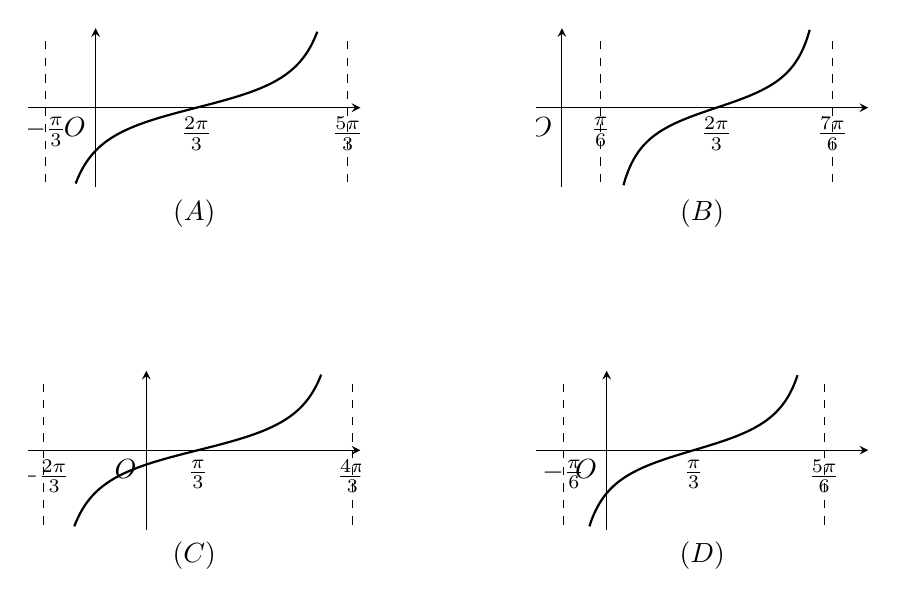
\begin{tikzpicture}[>=stealth]
  % (A)
  \begin{axis}[
    width=5.8cm, height=3.6cm,
    axis lines=middle, xmin=-1.4, xmax=5.5, ymin=-3.2, ymax=3.2,
    xtick=\empty, ytick=\empty, samples=240,
    restrict y to domain=-3.15:3.15, unbounded coords=jump,
    clip=true, title={$(A)$},
    title style={at={(axis description cs:0.5,-0.12)}, anchor=north},
  ]
    \addplot[thick, domain=-0.98:5.17]
      {tan(deg(0.5*x-pi/3))};
    \draw[dashed] (axis cs:-1.047,-3)--(axis cs:-1.047,3)
      (axis cs:5.236,-3)--(axis cs:5.236,3);
    \node[below] at (axis cs:-1.047,0) {$-\frac\pi3$};
    \node[below] at (axis cs:2.094,0) {$\frac{2\pi}3$};
    \node[below] at (axis cs:5.236,0) {$\frac{5\pi}3$};
    \node[below left] at (axis cs:0,0) {$O$};
  \end{axis}

  % (B)
  \begin{axis}[
    at={(6.45cm,0)}, anchor=south west,
    width=5.8cm, height=3.6cm,
    axis lines=middle, xmin=-0.35, xmax=4.15, ymin=-3.2, ymax=3.2,
    xtick=\empty, ytick=\empty, samples=240,
    restrict y to domain=-3.15:3.15, unbounded coords=jump,
    clip=true, title={$(B)$},
    title style={at={(axis description cs:0.5,-0.12)}, anchor=north},
  ]
    \addplot[thick, domain=0.58:3.61]
      {tan(deg(x-2*pi/3))};
    \draw[dashed] (axis cs:0.524,-3)--(axis cs:0.524,3)
      (axis cs:3.665,-3)--(axis cs:3.665,3);
    \node[below] at (axis cs:0.524,0) {$\frac\pi6$};
    \node[below] at (axis cs:2.094,0) {$\frac{2\pi}3$};
    \node[below] at (axis cs:3.665,0) {$\frac{7\pi}6$};
    \node[below left] at (axis cs:0,0) {$O$};
  \end{axis}

  % (C)
  \begin{axis}[
    at={(0,-4.35cm)}, anchor=south west,
    width=5.8cm, height=3.6cm,
    axis lines=middle, xmin=-2.4, xmax=4.35, ymin=-3.2, ymax=3.2,
    xtick=\empty, ytick=\empty, samples=240,
    restrict y to domain=-3.15:3.15, unbounded coords=jump,
    clip=true, title={$(C)$},
    title style={at={(axis description cs:0.5,-0.12)}, anchor=north},
  ]
    \addplot[thick, domain=-2.03:4.12]
      {tan(deg(0.5*x-pi/6))};
    \draw[dashed] (axis cs:-2.094,-3)--(axis cs:-2.094,3)
      (axis cs:4.189,-3)--(axis cs:4.189,3);
    \node[below] at (axis cs:-2.094,0) {$-\frac{2\pi}3$};
    \node[below] at (axis cs:1.047,0) {$\frac\pi3$};
    \node[below] at (axis cs:4.189,0) {$\frac{4\pi}3$};
    \node[below left] at (axis cs:0,0) {$O$};
  \end{axis}

  % (D)
  \begin{axis}[
    at={(6.45cm,-4.35cm)}, anchor=south west,
    width=5.8cm, height=3.6cm,
    axis lines=middle, xmin=-0.85, xmax=3.15, ymin=-3.2, ymax=3.2,
    xtick=\empty, ytick=\empty, samples=240,
    restrict y to domain=-3.15:3.15, unbounded coords=jump,
    clip=true, title={$(D)$},
    title style={at={(axis description cs:0.5,-0.12)}, anchor=north},
  ]
    \addplot[thick, domain=-0.46:2.55]
      {tan(deg(x-pi/3))};
    \draw[dashed] (axis cs:-0.524,-3)--(axis cs:-0.524,3)
      (axis cs:2.618,-3)--(axis cs:2.618,3);
    \node[below] at (axis cs:-0.524,0) {$-\frac\pi6$};
    \node[below] at (axis cs:1.047,0) {$\frac\pi3$};
    \node[below] at (axis cs:2.618,0) {$\frac{5\pi}6$};
    \node[below left] at (axis cs:0,0) {$O$};
  \end{axis}
\end{tikzpicture}
